\begin{frame}{今回の改善点}
 
    \begin{columns}[t]
    \begin{column}{0.7\textwidth}
        <今回の改善点> \\
         \begin{itemize}
            \item[①] コンター図がまだら模様の件 \\
                     これは4面体メッシュでの解析ではやむを得ない \\
                     \Add{6面体メッシュ}を用いてメッシュを切りなおす
            \item[]
            \item[②] 薄肉構造を仮定した件 \\
                     板厚方向に多くの分割数を確保し \\
                     板厚方向の\Add{応力分布}を\Add{厚肉円筒の応力式}と比較
            \item[]
            \item[③] メッシュ数の節約のため、\\
                     1/8ショートケーキモデルとする
         \end{itemize}
    \end{column}
    \begin{column}{0.3\textwidth}
      \begin{figure}[htbp]
        \begin{center}
          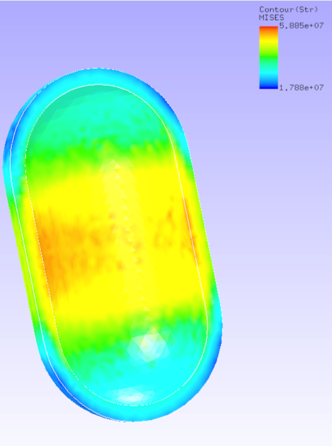
\includegraphics[keepaspectratio,scale=1.5]{work/images/previous.png}
            \caption{以前の勉強会で報告された結果(再掲)}
        \end{center}
      \end{figure}
    \end{column}
  \end{columns}
  %
  % TiKZを使った図形の描画 図2でA点を指し示す矢印
  \begin{textblock*}{30pt}(385pt,95pt)
    \begin{tikzpicture}
        \draw[->, draw=cud_red, line width=2pt] (0.7,0.8) -- (0,0.3);
        \node[rectangle,fill=cud_yellow,text width=0.5cm,text centered,rounded corners,minimum height=0.5cm](s) at (1cm,1cm) { \scriptsize A点};
    \end{tikzpicture}
  \end{textblock*}
\end{frame}
